
\section{Data Structure}
\label{sc:datastructure}
\subsection{Bucket}
\label{ssc:bucket}
The most elementary data object is the \textit{bucket}. Each and every submitted item is submitted in a bucket: datasets, paragraphs, images and formulae are contained in buckets. These are examples of \textit{atomic buckets}, expressing the fact that they are the building blocks of the system. 
% We decisively opted against objects that represent traditional folders, where every file belongs to one and only one folder\footnote{In git the folder object is called a \textit{tree node} and it is not possible for a file (called a \textit{blob} in git-speak) to belong to multiple trees. In the unix filesystem it is only possible through the hack of soft and hard links.}.
Instead of a folder structure we solve the containment relation through designated buckets that we call \textit{molecular buckets} (like \textit{tree} nodes in git). The data part of those buckets contains merely an arrangement of atomic buckets. One may think of them as the analogue of an article, a book or some other curated content. 


\begin{figure}[h!]
  \begin{center}
    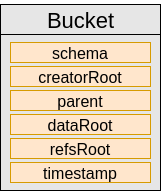
\includegraphics[width=0.20\textwidth]{src/img/DataBucketV2.png}
\end{center}
 \caption{The most elementary type of data container is the bucket. It contains only immutable entries (orange), such as the \textit{schema}, the \textit{creatorRoot}, the \textit{parent}, the \textit{dataRoot}, the \textit{refsRoot} and the \textit{timestamp}.}
 \label{fig:bucket}
\end{figure}


Every bucket contains six entries: A \textit{schema}, a \textit{creatorRoot}, a \textit{parent}, a \textit{dataRoot}, a \textit{refsRoot} and a \textit{timestamp}. See Figure \ref{fig:bucket} for an illustration. Here and henceforth the word root refers to the root of a Merkle tree. We go through the entries in turn. The \textit{schema} contains information about the format of the data. For instance we have already mentioned that the data in the molecular buckets is formatted as an arrangement\footnote{The purposefully vague formulation of an 'arrangement' is due to the intention to keep that format flexible. One may think of this as an ordered list, but one might also consider further directives or clustering of content in a directed hypergraph.}. The \textit{creatorRoot} points to information about the creator of this bucket. Identity on \textit{Lakat} is solved through proofs (see Section \ref{ssc:proofs}). The \textit{parent} is the \textit{content identifier} of the parent bucket. For genesis buckets that would be 0. The \textit{dataRoot} is a content identifier of the data contained in the bucket. In future versions the schema could be absorbed into the dataRoot using the ipld multihash format. This would require a Lakat-specific codec. The \textit{refsRoot} points to all the references made to other buckets within the data. This is necessary, since references to other buckets might be obscured inside the data-encoding. This is an analogue of a list of citations. The \textit{timestamp} records the time of inclusion of the bucket into the branch. It is important to note that we use ethereum block hashes as time stamps in our first version, since the local consensus is too weak to ensure that all participants are truthful to the time otherwise. Anticipating block hash is close to impossible. One cannot change the data inside the bucket. One would have to create a new bucket that points to the original bucket via its parent entry. 




\subsection{Branch}
\label{ssc:branch}

\begin{figure}[t!]
\begin{center}
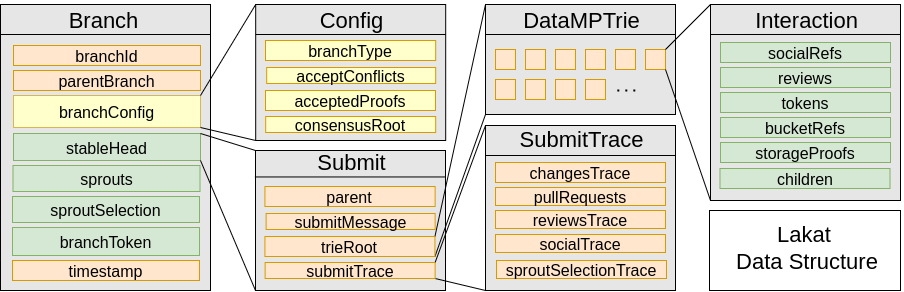
\includegraphics[width=\textwidth]{src/img/BranchV9.png}
\end{center}
 \caption{A schematic illustration of the branch object and its entries.}
 \label{fig:branchstructure}
\end{figure}
The central object type of Lakat is the \textit{branch}. See Figure \ref{fig:branchstructure} for an illustration. Branches represent journals or research communities. They share some properties with \textit{git}-branches and some with blockchains. Every branch contains an id, called \textit{branchID}, that uniquely identifies it. The immutable entries of a branch and the initial head are hashed to produce the branch identifier. The branch also points to a parent branch from which it was branched off. This entry may however be empty for a certain type of branch, namely the sprout (see below). The corresponding entry is called \textit{parentBranch}. This construction turns the set of branches into a linked data structure.\footnote{\remark{Maybe check this} In \textit{git} a branch is simply pointer to the head commit. In blockchains one often encounters ids attached to the chain (so-called \textit{chainid}) to avoid issues when the consensus mechanism yields two differnt chains.} At creation time the branch receives a \textit{timestamp}. The previous entries are all immutable. There are then four mutable entries, namely \textit{stableHead}, then the two consensus entries \textit{sprouts} and \textit{sproutSelection} and finally \textit{branchToken}. The stable head is a pointer to the latest stable submit. A \textit{submit} is a set of changes (see Subsection \ref{ssc:submit} on submits). One may think of it as the Lakat version of an article submission. It has similiarities to a commit in git -- not only phonetically -- but also to a block in \textit{ethereum}. The addition of new submits works through a consensus mechanism called \textit{proof of review (PoR)} and \textit{lignification} (see Subsection \ref{ssc:consensus}). Also in this respect the branch behaves a lot like a blockchain. Every branch has it's own token, the \textit{branchToken}. It allows funding bodies to fund a particular branch. Token logic is not handled by \textit{Lakat}. Instead this entry essentially points to proofs of transactions on a blockchain where the respective token lives. The purpose of the integration of tokens is to create an incentive layer on top of Lakat, because (unfortunately) \textit{humans} as well as \textit{AI} do not work without incentives. The branch also carries configurational metadata, stored in \textit{branchConfig}. It points to information about the branch type, whether merge conflicts are accepted (see Subsection \ref{ssc:submit}), the consensus rules and the proofs that are accepted, such as proofs of token transfer or proofs of time. We use timestamps from latest blocks on various blockchains as proofs of time (see \cite{gipp2015decentralized} and also  \href{https://opentimestamps.org/}{opentimestamps.org}). The branchConfig's mutability is more constrained than that of the stable head (See Subsection \ref{ssc:configchange}).
Finally, we envision a way to extend the config schema. This would be done by an additional entry that points to a \textit{schema bucket}, where the schema for the config is defined. An empty entry would signify the use of the default schema.


There are three types of branches: \textit{proper branches}, \textit{sprouts} and \textit{twigs}. The branch type is stored in the branch config and can be changed under certain conditions. 
\textit{Proper branches} can only be modified through the local consensus mechanism (see Subsection \ref{ssc:consensus}). They point to a non-empty set of sprouts, which help with the process of producing stable heads in the proper branch. Proper branches cannot be changed to any other branch type. A \textit{sprout} is a short-lived branch that is exclusively used to grow proper branches. Sprouts behave a bit like ommers in the ethereum protocol in the sense that they are contestors to produce the next stable head. They do not have an empty parent branch entry. Sprout branches point to an empty set of sprouts themselves. The sproutSelection contains all the sprouts that are rooted in it. The branchToken entries is empty. The stableHead is immutable. There is only one way to modify the sprout, namely indirectly when it turns into a proper branch during the lignification process (See Subsection \ref{ssc:lignification}). Once a sprout turns into a proper branch the parent branch entry is filled with the id of the branch that it is rooted in. Finally, a \textit{twig} can be thought of a little feature branch. Twigs can be modified through submits by \textit{contributors} of the twig (See Subsection \ref{ssc:contributors} for more information on contributors) or through merges. However, the process of merging into a twig does not need to go through the consensus mechanism of proper branches (See Subsection \ref{ssc:consensus}).

In this paragraph we merely introduce some nomenclature. We distinguish between \textit{core} and \textit{belt} branches, which correspond to \textit{this} and \textit{other} in git. These are not intrinsic properties of branches, but denote the role they play during a merge. Lakat only has one type of merge. The core branch will be updated and the belt branch not (see Susbsection \ref{ssc:merge} for information on merges). A branch may be a core with respect to one merge and a belt with respect to another merge. This terminology originates in the core-belt dichotomy of Lakatosian research programmes. There is a further distinction that is purely conceptual and is not manifested in the technical specification, but in the nomenclature. We distinguish a \textit{derived branch} from a \textit{seedling branch} in that the seedling branch has a \textit{singularity submit} without a parent (See Subsection \ref{ssc:submit} for information on submits). A singularity submit corresponds to the genesis block in a blockchain. We invoke here a cosmological metaphore rather than a biblical one. The seedling branch has no parent branch and the corresponding entry points to zero. A derived branch on the other hand has a parent branch that it points to. We say that the derived branch is \textit{rooted} in the parent branch. The \textit{root} of a derived branch is the last submit in the submit history that is also in the history of the parent branch.

We also not that there are various levels at which Lakat can be viewed as a graph, going from high level to low level. At the level of the branches one can form a graph $\mathcal B$, where a branch is a node and a directed link from one branch $A$ to another branch $B$ means that $B$ is the parent of $A$ or that $B$ is merged into $A$ (See Subsection \ref{ssc:merge} regarding merging). This directed graph is not necessarily a-cyclic, because $A$ can be rooted in $B$ and merge back into $B$, however if one excludes merges it is. At the level of the submits, a graph $\mathcal S$ can be created with the submits being nodes and a link can be drawn from a submit $q$ to $p$ when $p$ is the parent of $q$. This yields a directed acyclic graph (DAG). Finally at the level of the data buckets there exists a graph structure $\mathcal D$ induced by the parent reference inside the bucket. There is a graph homomorphism from $\mathcal S$ to $\mathcal B$, but not vice versa and there are no homomorphisms between $\mathcal S$ and $\mathcal D$ or $\mathcal B$ and $\mathcal D$. The lack of a homomorphism between the submit structure and the data structure indicates that these are two separate layers. The relation between the elementary bucket object and the higher level branch object is not simply a many-to-one relation. Different branches may share the some data buckets. In practice one would expect that most of the data inside a branch is shared with at least one other branch. See Figure \ref{fig:branchbucketrel} for an illustration of this relation.



\subsection{Submit}
\label{ssc:submit}
Submits bundle up changes to the data with some additional metadata. Every submit points to a previous submit, the \textit{parent} submit. There exist \textit{singularity} submits that have no parent. The parent entry of those submits is zero. Like in git or ethereum, there is a field reserved for submit-specific data that we call \textit{submitMessage}. The change of the data within the submit is subsumed in \textit{trieRoot}, which is the root of the \textit{DataMPTrie}, a Merkle-Patricia-Trie that references the data state of Lakat (see Section \ref{ssc:datatrie}). The leafs of the trie are the data buckets. They have some resemblance with accounts in the ethereum state trie. Usually only a small part of the entire trie gets updated in a submit. Imagine the trie being all of wikipedia and a submit being just the creation of a new page or even just editing a page. Event though the bucket identifier is immutable it points to mutable entries. This is similar to ethereum, where the leave nodes are immutable account addresses that point to mutable entries like amount of ETH, the contract storage data or the account nonce. The mutable entries in the case of Lakat are made up of information that is attached by other users to the bucket. It is information that is not intrinsic to the bucket. This includes \textit{socialRefs}, \textit{reviews}, \textit{tokens}, \textit{bucketRefs} and \textit{storageProofs}. 

The socialRefs resolve to tokens of appreciation, such as thumbs up or down -- the gold standard of social media user interaction. The reviews point to data buckets that contain a review or comments on the bucket in question. The tokens entry allow for the integration of tokens to data buckets. The bucketRefs are two collections of references to other buckets. The first collection is immutable and contains all those other buckets that are referenced inside the bucket data. This second collection is mutable and consists of all those molecular buckets that the atomic bucket is part of. This is a reverse registry that can be understood as how much a content has been reused. There is no analogue in classical publishing. StorageProofs are a ledger of timestamped proofs of storage for the bucket.  

There are some submits with a specific structure. These are the \textit{pull requests} (see Subsection \ref{ssc:por}) and the merge submits (see Subsection \ref{ssc:branchops}). The pull request  contains at least one context bucket, called the \textit{review container}, that references all the subsequent reviews. It also leaves a trace of the pull request in the submitTrace. The merge submit contains 
all the data buckets of the belt branch and it points to the merged branch id in the submitTrace. 

In Lakat conflicts are at the heart of the protocol. They are cherished as the source of progress and sets Lakat apart from conventional publishing systems. We provide a clear definition of a conflict. A \textit{submit conflict} with respect to a branch $\mathfrak B$ is a set 
of three submits $\pi$, $s_1$ and $s_2$ where $\pi$ is the parent of both $s_1$ and $s_2$ and all three are included in $\mathfrak B$. We denote this 4-tupel by $(\mathfrak B, \pi, s_1, s_2)$.
A submit that creates a submit conflict is called a \textit{conflicted submit} and a submit that does not create a submit conflict is called \textit{conflictless submit}.
A \textit{merge conflict} is a submit conflict that arises from a merge submit. Depending on the branch configuration (see Subsection \ref{ssc:branch}) merge submits may or may not bring about merge conflicts. 


\subsection{Data--Trie}
\label{ssc:datatrie}

The data buckets as well as the mutable information attached to them can be looked up with the help of a Merkle-Patricia trie, called the \textit{DataMPTrie}. This is cryptographically secure and very useful when resolving the information attached to buckets inside of an article. The keys that are stored in the trie are a truncated version of the content identifiers of the data buckets. And the values are the mutable entries attached to the buckets. To look up the bucket data itself one uses simply the content identifier of the bucket. Storage is handled separately (see Storage in Section \ref{ssc:storage}).
We propose to use a modified Merkle-Patricia trie -- very similar to the one used in Ethereum -- with four types of nodes: null nodes, leaf nodes, extension nodes and branch nodes \cite{}.
The data at each node is serialized and hashed. The specifics of this encoding are yet to be specified. One may use any of the existing ipld-formats. The encoding should have the property that data lists with a lot of empty entries are serialized in a very compact way to save space. Many data items in Lakat have a lot of empty fields. A bucket without any interaction information is mostly empty fields. A twig or a sprout have many empty fields as well. The leaf-nodes (in the trie) are special in this respect, because the hashing uses a salt that equals the content identifier of the bucket. Why do we need a salt at all? When a data bucket is published it doesn't have any information attached to it, so without the salt all new data buckets would have the same hash, which is not desirable.





\begin{figure}[b!]
  \begin{center}
    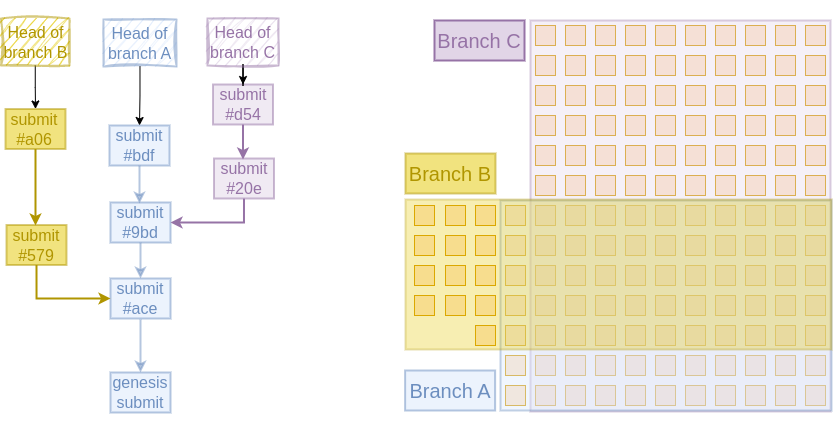
\includegraphics[width=1.0\textwidth]{src/img/BranchBucketRelationV2.png}
\end{center}
 \caption{}
 \label{fig:branchbucketrel}
\end{figure}

\subsection{Storage}
\label{ssc:storage}

% i
The data is stored in key-value databases and is content addressed in the sense that the key equals the multihash of the data. We would like to use the ipld standard for linked data. Inside the multihash there is information about the storage protocols where the data is stored and can be retrieved. A piece of data can be stored with multiple protocols. A contributor may also choose to store the information on the own machine of course at the risk of having reduced uptime and not being discoverable. If one would use ipfs for storage then a certain flag in the multihash would be raised. If also another protocol or system would be used then this would again be seen through the flag in the multihash. The more branches point to a piece of data and the more subsequent submits rely on it the more important the persistence of that data becomes.   
The idea is that the availability, the longevity and the redundancy of data will scale with its importance in a self-organized fashion. A branch with many contributors will make sure to have the storage well secured and also well distributed. A newly created branch on the other hand needs to broadcast its creation (see Subsection \ref{ssc:branchrequests} for branch creation broadcasting) to allow for distributed storage  and attract contributors to ensure decentralized persistence of its data. 
This has two advantages. 1) Data that is pointed at by many branches is highly available and more redundant. 2) One cannot attack the system by creating lots and lots of branches. To proof that a certain data bucket has been stored, i.e. pinned, that proof is attached to the mutable information of the bucket in the \textit{storageProofs} entry. There are a few more constraints about storage and pinning. It should be encouraged that every data bucket belongs to at least one molecular bucket so that there are no buckets without a context. Thus when a new data bucket is submitted the submission won't be accepted unless it is present in at least one context bucket.

When a new branch is created the data is initially just stored by the branch creator, but broadcasted through the network. Some nodes may pick up the data and store it as well. The branch creator may also choose to pin the data bucket in a certain storage system. Data that is close in the branch data structure is also close in the storage system. This is a very important feature of Lakat. It allows for a very efficient retrieval of data. The storage of data pertaining to a branch can be rewarded in branch tokens. This is not a feature of Lakat, but may be added on top of it to incentivize storage. There may also be a market for storage, where branch creators can buy storage space for their branch data. This is also not a feature of Lakat, but may be added on top of it.

\subsection{Branch--Requests}
\label{ssc:branchrequests}

Every branch has its own staging area, where any type of branch interactions are waiting to be included. This is called the \textit{Branch--Requests} (or BR in short). It is similar to the mempool in ethereum. Everyone who is participating in the branch (See Protocol \ref{ssc:protocol}) and who runs a light client may receive branch interactions from users and broadcast them to the network. Here we refer to a \textit{client} as a piece of software that is yet to be written, which interacts with the network. A \textit{light client} is a client that is not capable of doing branch operations, but is capable of receiving and broadcasting branch--requests. Inclusion of requests into the branch, however, requires more (see Protocol \ref{ssc:protocol}). There are eight channels in the branch--requests (see Figure \ref{fig:mempool}): \textit{submit requests}, \textit{pull requests}, \textit{review commits}, \textit{review submit requests}, \textit{social transactions}, \textit{token transactions}, \textit{storage updates} and \textit{branch creation broadcast}. The requests inside the BR are not permanently stored. Requests are kept for as long as any of the branch contributors keeps track of them. That is where the similarity to the mempool stems from.

Every channel in the Branch Requests has a certain capacity. In particular this aims to prevent that one channel clutters the entire pool of requests, which might happen if the capacity was channel-independent. All requests or broadcasts are serialized. 
Submit requests contain a serialization of the data buckets that are requested to be added to the branch. Pull requests are simply pings from other branches that seek reviewers. Only by means of a pull request are contributors from the target branch allowed to make modifications to the requesting branch (see Proof of Revie \ref{ssc:consensus}).


\remark{One can submit interaction data to any branch that holds it. Once a branch processes it, }



\begin{figure}[h!]
  \begin{center}
    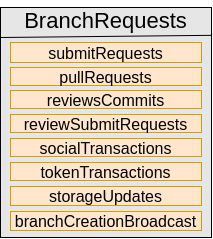
\includegraphics[width=0.25\textwidth]{src/img/MempoolV3.png}
\end{center}
 \caption{}
 \label{fig:mempool}
\end{figure}
